%%%%%%%%%%%%%%%%%%%%%%%%%%%%%%%%%%%%%%%%%%%%%%%%%%%%%%%%%%%%%%%%%%%%%%%%
%    INSTITUTE OF PHYSICS PUBLISHING                                   %
%                                                                      %
%   `Preparing an article for publication in an Institute of Physics   %
%    Publishing journal using LaTeX'                                   %
%                                                                      %
%    LaTeX source code `ioplau2e.tex' used to generate `author         %
%    guidelines', the documentation explaining and demonstrating use   %
%    of the Institute of Physics Publishing LaTeX preprint files       %
%    `iopart.cls, iopart12.clo and iopart10.clo'.                      %
%                                                                      %
%    `ioplau2e.tex' itself uses LaTeX with `iopart.cls'                %
%                                                                      %
%%%%%%%%%%%%%%%%%%%%%%%%%%%%%%%%%%
%
%
% First we have a character check
%
% ! exclamation mark    " double quote  
% # hash                ` opening quote (grave)
% & ampersand           ' closing quote (acute)
% $ dollar              % percent       
% ( open parenthesis    ) close paren.  
% - hyphen              = equals sign
% | vertical bar        ~ tilde         
% @ at sign             _ underscore
% { open curly brace    } close curly   
% [ open square         ] close square bracket
% + plus sign           ; semi-colon    
% * asterisk            : colon
% < open angle bracket  > close angle   
% , comma               . full stop
% ? question mark       / forward slash 
% \ backslash           ^ circumflex
%
% ABCDEFGHIJKLMNOPQRSTUVWXYZ 
% abcdefghijklmnopqrstuvwxyz 
% 1234567890
%
%%%%%%%%%%%%%%%%%%%%%%%%%%%%%%%%%%%%%%%%%%%%%%%%%%%%%%%%%%%%%%%%%%%
%

%\documentclass[12pt]{iopart}
\documentclass[12pt]{article}
%\usepackage{amsmath}
\usepackage{cite}
\usepackage{amsmath,amssymb,amsfonts}
\usepackage{algorithmic}
\usepackage{graphicx}
\usepackage{textcomp}
\usepackage{xcolor}
\usepackage{graphicx}
%Uncomment next line if AMS fonts required
%\usepackage{iopams}  
\begin{document}

\title{Optogenetic Maxwell Demon to Exploit Intrinsic Noise and Control Cell Differentiation Despite Time Delays and Extrinsic Variability}
\maketitle

\author{M P May$^1$, B Munsky$^{1,2}$}

%\address{$^1$ School of Bioengineering, Colorado State University, Fort Collins, Co}
%\address{$^2$ Dept. of Chemical and Biological Engineering, Colorado State University, Fort Collins, Co}

%\vspace{10pt}
%\begin{indented}
%\item[]August 2017
%\end{indented}

\begin{abstract}
Synthetic biology seeks to create modular components that generate complex and controllable biological behaviors, often at microscopic scales. In single-cell applications, where important regulatory RNA or proteins are present in small numbers, intrinsic fluctuations cause biochemical `noise' that frequently results in undesired effects, and this noise is usually treated as a nuisance that must be removed. However, recent theoretical analyses have shown that noise can sometimes be used to one's advantage when seeking to manipulate nonlinear regulatory systems that would be difficult or impossible to control in a fully deterministic setting. Specifically, it was shown that a noise-exploiting optogenetic controller reminiscent of Maxwell's Demon could systematically force multiple identical systems to reach different independently-assigned stable points, even for a few special cases where the model is inexact or if observations were incomplete. This work expands upon those analyses to explore in greater detail how control performance is affected by errors or approximations in the model or by temporal delays in the observations. We find that noise-exploiting controllers can remain highly effective despite coarse approximations to the model's scale or incorrect estimations of key model parameters, and these controllers can even retain performance for significant time delays.  Together, these findings suggest that noise-exploiting control should be possible in real experiments where models are always approximate, where parameters are always uncertain, and where observations are corrupted by errors.

\end{abstract}
Keywords: Optogenetic control, Stochastic gene regulation, Synthetic biology

%
% Uncomment for keywords
%\vspace{2pc}
%\noindent{\it Keywords}: Stochastic control, optogenetic, synthetic biology
%
% Uncomment for Submitted to journal title message
%\submitto{\JPA}
%
% Uncomment if a separate title page is required
\maketitle
% 
% For two-column output uncomment the next line and choose [10pt] rather than [12pt] in the \documentclass declaration
%\ioptwocol

\section{Introduction}
\begin{figure}
\begin{center}
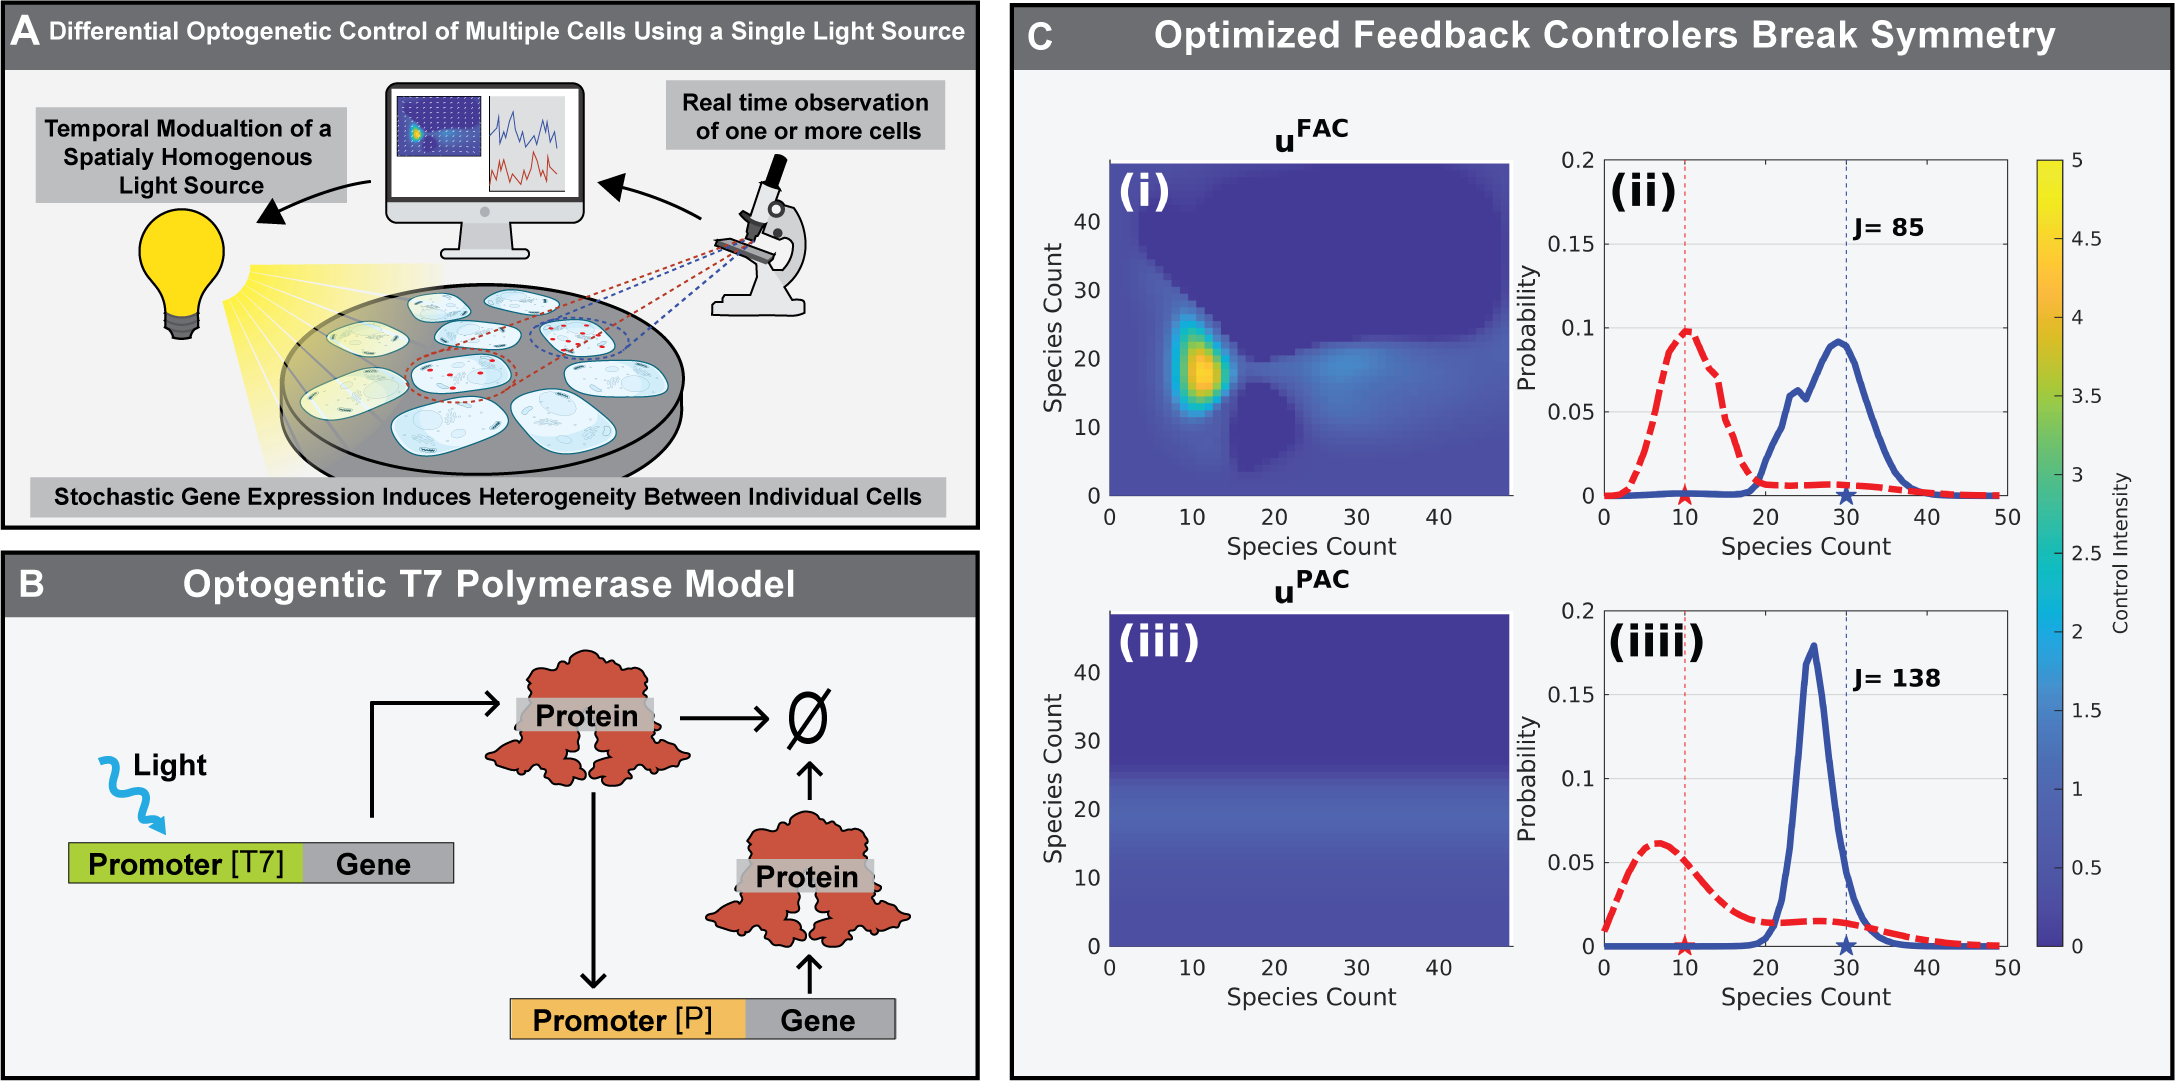
\includegraphics[width=\columnwidth]{CartoonAndControler.png}
\caption{(A) Schematic of the T7 optogenetic control system (adapted from \cite{May2021}). A microscope observer is partially (PAC) or fully (FAC) aware  of cells; the resulting controller modulates a single spatially homogeneous light signal that perturbs all cells equally seeks to drive each genetically identical cells to a different, specified states. (B) Schematic of the optogenetically controllable T7 polymerase model, which is identical in all cells: Light activates the T7 polymerase-based production of protein, and the protein self-actuates its own production. (C) The FAC (top) and PAC (bottom) control laws for two cells ($\mathbf{u}^{XAC}(x_1,x_2)$ shown on left) break the symmetry between Cell 1 and Cell 2 and result in distinct marginal distributions for the cells' responses (right).}
\label{cartoons}
\end{center}
\vspace{-0.3in}
\end{figure}


Synthetic biology seeks to create modular\cite{Ng2019} and orthogonal\cite{Liu2018} components to sense and actuate\cite{Sheets2020} complex logical systems\cite{Groseclose2020}, and which are capable of performing a variety of advanced biological behaviors\cite{Shin2020}. 
New optogenetic tools have increased our ability to actuate embedded systems within cells reliably and with strong control performance\cite{Sheets2020,Baumschlager2017,Chen2020,Lillacci2018}. Great advances in these two fields have enabled computer programmable control of cellular protein production through the use of external optogenetic inputs and smart microscope techniques\cite{Fox2021,Baumschlager2021,Lugagne2017}. These types of digital-synthetic actuators allow for fine-tuned, computer-modulated control of cellular systems that were previously impossible\cite{Rullan2018, Baumschlager2017} and with fast response times in comparison to chemical diffusion. 

Classical and modern control methods like PID control and model predictive control have been implemented in such systems\cite{} which can control synthetic systems to different stable points. Theoretical works have shown that stochastic systems can be controlled to unstable points by oscillating around those points \cite{Guarino2020} but new control techniques which exploit the full probability distribution information of the system can be used in certain scenarios to control simple systems to unstable points by exploiting the natural noise of protein production to its advantage. Previous control effort focus on deterministic ODE formulations of the control problem, but only a few studies seek to analyze the full chemical master equation to exploit noise to {\em improve} the control of synthetic biology processes \cite{Szymanska2015,May2021}.  

In \cite{May2021}, it was surprisingly found that, when noise, auto-regulation, and noise-exploiting feedback control were all present at once, the system could be controlled to bring two similar cells to two different arbitrary points simultaneously (Figure \ref{cartoons}A), but when any one of these components were missing the system could not break its symmetry. More specifically, this required that the symmetry between the protein probability distributions of each cell would not be not the same (or asymmetric). Three effective controllers were found which could do this, a Fully Aware Feedback Controller (FAC) that observed the protein counts of all observed cells, a Partially Aware Feedback Controller (PAC) that observed the protein counts of only one cell, and a probabilistic Model Predictive Feedback Controller (pMPC) that observed only the primary cell and integrated a probabilistic model to represent the non-stationary probability distribution of the secondary cells in the same environment. 

The solutions of the controllers was carried out by solving the chemical master equation (i.e., the forward Komogorov equation) to estimate the probability of possible cellular states. For a two cell, single-input-single output (SIMO) control problem, the FAC performed the best (figure\ \ref{cartoons}C(top)), and the PAC (figure\ \ref{cartoons}C(bottom)) 2nd, and pMPC controllers 3rd. In all cases, the controller's knowledge and explicit treatment of intrinsic noise was critical to improve the control performance, break symmetry, and enable the SIMO control of all cells.

In this paper, the control problem is extended to examine how the FAC and PAC controllers are affected by time delay, the system granularity, and parameter uncertainty. In the `Methods' section, we briefly set up a stochastic chemical master equation model for multiple individual cells in the same spatially homogeneous environment, and we formulate the effects of FAC and PAC controllers on the dynamics of cells within that environment. Next, in the `Results' section, we examine the effects of volume changes, time delays, and parametric uncertainties on the FAC and PAC control performance. Finally, in `Conclusions' we summarize our findings and discuss potential implications that these controllers may have on future systems and synthetic biology investigations.

\section{Methods}
We begin with a five species model for the production of an arbitrary protein through the activation of light activatible T7 polymerase (figure 1B) motivated by Baumschlager, et al.
This model for the production of protein uses a split T7 domain ($T7_N$,and $T7_C$) which reversibly dimerizes in the presence of light to create a T7 dimer. The T7 monomer is created at a constant rate and degrades linearly with the number of monomer. The split monomers of T7 can bind to create a T7 dimer (equation ...) . The T7 dimer can then bind to a gene which enables the production of protein with a leak term, and the protein can bind to a secondary self-activated promoter described by a Hill function for the creation of more protein. This auto-regulatory motif in protein production is responsible for creating non-linearity in the system that enables noise-exploiting control. The final step was the degredation of protein 

These model dynamics were then simplified to a single ODE with auto-regulation describing the protein accumulation as: 
\begin{equation}
\frac{dp}{dt}=u(x_1,x_2)  + \kappa\frac{p^\eta}{p^\eta+\beta^\eta}+ k_0 -\gamma p,
\label{rateeq}
\end{equation}

where $p$ is the protein count; $\kappa$ is the maximum auto-regulation promoter strength; $\beta$ is the concentration at which auto-regulation reaches half strength; $\eta$ is the auto-regulation promoter cooperativity; $\gamma$ is the degradation rate; $k_0$ is the promoter leakage rate; and $u$ is the T7 promoter strength.  The protein production rate response to the light level $u$ can be modulated in response to the state of the system $u(x_1,x_2)$ and introduces the possibility of state-dependent optogenetic feedback to the system.  We note that $u(x_1,x_2)$ refers to the effect of light on the optogenetic system instead of light activity itself. A schematic of the model is shown in figure \ \ref{cartoons}B, and parameters were chosen to reproduce dynamics measured in \cite{Baumschlager2017} and are shown in are defined in Table 1\cite{May2021}. Two optimized controls laws $u=u^{\rm (FAC)}$ and $u=u^{\rm (PAC)}$ are depicted in figure \ \ref{cartoons}C (top left and top right, respectively).


\begin{table}[]
\caption{Model Parameters}
\begin{center}
\begin{tabular}{|c|c|c|}
\hline
Parameter & Value   & units                     \\ \hline
$\kappa$         & 0.406   & Molecules Per Minute \\
$\beta$          & 20.0    & Molecules            \\
$\eta $           & 8.00    & unit less          \\
$k_0$           & 0.0001  & Molecules per Minute \\
$\gamma$         & 0.0203  & per Minute         \\
$u$              & dynamic & Molecules per Minute \\ \hline
\end{tabular}
\label{table}
\end{center}
\vspace{-0.2in}
\end{table}

\subsection{Stochastic Simulation Algorithm and the Finite State Projection}
Solving discrete stochastic representations of chemical dynamics is critical to the development of noise-exploiting controllers, and can be analyzed using the Stochastic Simulation Algorithm (SSA) , or the Finite State Projection (FSP).
To recast the above ODE formulation into the discrete stochastic representation, we define the enumerated $i = 1,2,\ldots$ states of the system as the tuple of the numbers of proteins in each cell as $\mathbf{X}_i = [x_{i1},x_{i2},\ldots,x_{iN_c}]$, and we define the stoichiometry vectors as the change in state following one reaction event (e.g., $\mathbf{X}_i \rightarrow \mathbf{X}_i + \mathbf{s}_\nu$), where the $2N_c$ possible reactions are:
 
\begin{align}
\mathbf{s}_1 &= \mathbf{e}_1,\ \mathbf{s}_2 = -\mathbf{e}_1,\nonumber\\ 
\mathbf{s}_3 &= \mathbf{e}_2,\ \mathbf{s}_4 = -\mathbf{e}_2,\nonumber\\
&\vdots \nonumber\\ 
\mathbf{s}_{\rm 2N_c-1} &= \mathbf{e}_{\rm N_c},\ \mathbf{s}_{\rm 2N_c} = -\mathbf{e}_{\rm N_c}, \label{Stochs}
 \end{align}
 
 
where each $\mathbf{e}_{i_c}$ corresponds to the Euclidean basis vector for the $i_c^{\rm th}$ cell. The corresponding propensity functions are:
\begin{align}
w_1 &= u(\mathbf{X},t)  + \kappa \frac{x_1^\eta}{x_1^{\eta}+\beta^{\eta}} + k_0,\ w_2 = \gamma x_1,\nonumber\\
w_3 &= u(\mathbf{X},t)  + \kappa \frac{x_2^\eta}{x_2^{\eta}+\beta^{\eta}} + k_0,\ w_4 = \gamma x_2,\nonumber\\
&\vdots \nonumber\\
w_{\rm 2N_c-1} &= u(\mathbf{X},t)  + \kappa \frac{x_N^\eta}{x_N^{\eta}+\beta^{\eta}} + k_0,\ w_{\rm 2N_c} = \gamma x_N,\label{Props}
 \end{align}
With these stoichiometry and propensities, we can formulate and run the Gillespie stochastic simulation algorithm\cite{Gillespie1992,Gillespie1977} to generate representative trajectories of the stochastic process.

For the same specifications of the stoichiometry and propensity functions, the chemical master equation can also be formulated in matrix/vector form as:
\begin{equation}
\frac{d}{dt}\mathbf{P}=(\mathbf{A}_0+\textbf{Bu}^{\mathcal{C}})\mathbf{P},\label{CME}
\end{equation}
where $\mathbf{P} = [P(\mathbf{X}_1), P(\mathbf{X}_2), \ldots ]^T$ is the enumerated probability mass vector for all possible states of the system; $\mathbf{A}_0$ is the infinitesimal generator of the stochastic process due to the autoregulation promoter and degradation events;  $\textbf{u}^{\mathcal{C}} =[u^{\mathcal{C}}(\mathbf{X}_1), u^{\mathcal{C}}(\mathbf{X}_2), \ldots ]^T$ is the collection of state-dependent control inputs associated with each state; and $\textbf{Bu}^{\mathcal{C}}$ is the infinitesimal generator for the T7 promoter expression by which the effects of controller $\mathcal{C}$ are introduced into the process. 


 
The generator $\mathbf{A}_0$ can be constructed according to:
\begin{equation}
[\mathbf{A}_0]_{ij} = \left\{
\begin{array}{rl}
-\sum_{\nu =1}^{2N_c} w_{\nu}(\mathbf{X}_j), &\text{for }i=j,\\
w_{\nu}(\mathbf{X}_j), &\text{for }\mathbf{X}_i = \mathbf{X}_j+\mathbf{s}_\nu\\
0, & \text{otherwise,}
\end{array}\right. 
\label{InfA}
\end{equation}
and the infinitesimal generator $\mathbf{Bu}^{\mathcal{C}}$ of the controller is given by
\begin{equation}
[\mathbf{Bu^{\mathcal{C}}]}_{ij} = \left\{
\begin{array}{rl}
- N_c{u}^{\mathcal{C}}(\mathbf{X}_j), &\text{for }i=j,\\
{u}^{\mathcal{C}}(\mathbf{X}_j), &\text{for }\begin{array}{ll}\mathbf{X}_i =\mathbf{X}_j + \mathbf{e}_{i_c}, \\ \text{and } i_c = 1,\ldots,N_c\end{array}\\
0, & \text{otherwise,}
\end{array}\right.
\label{InfB}
\end{equation}
where ${u}^{\mathcal{C}}(\mathbf{X}_j)$ is the specification of the $\mathcal{C}$ controller in terms of the (partially observed) state.

For a given controller, the steady state of the system ($\mathbf{P}^*$) found by solving Eq.\ \ref{CME} is given by
\begin{equation}
\mathbf{P}^*=null(\mathbf{A}+\textbf{Bu}^{\mathcal{C}}).\label{SSDist}
\end{equation}


and the infinitesimal generator $\mathbf{Bu}^{\mathcal{C}}$ of the controller is given by




\subsection{Control Performance, Optimization, \& Design}
Score metrics of steady state distributions were made in order to enable optimization of the system by adjusting controllers. In the control of a SIMO stochastic system, a control input which tries to perfectly control one system will create increased noise in the other system because their inputs are shared. Therefore, a controller which strikes a balance between the two cells should be important when it is being optimized.

 The control performance ($J$), is defined as the expected steady state squared Euclidean distance of the process from a specified target ($\mathbf{T}$) state according to $E\{(\mathbf{X}-\mathbf{T})^2\}$. This score can be rewritten in terms of a precomputed set of linear weights ($\mathbf{C}$) and the steady state probability distribution ($\mathbf{P}^*$ from Eq.\ (\ref{SSDist})) given by
{\small \begin{align}
J&= \lim_{t\rightarrow \infty}\mathbb{E}\{|\mathbf{X}(t)-\mathbf{T}|_2^2\} \nonumber \\ 
&=\sum_{i,j,\ldots} P^*(x_1=i,x_2=j,\ldots) ((i-\mathbf T_1)^2 + (j-\mathbf T_2)^2 +\ldots)\nonumber  \\
&=\sum_{i,j,\ldots} P^*_{ij\ldots}(t)C_{ij\ldots} =\mathbf{C}\mathbf{P}^*
\label{Euclid}
\end{align}}
Where $J$ is a scalar, $\mathbf{C}$ is a vector of weights given by the Euclidian distance, and $\mathbf{P}^*$ the vectorized steady state distribution of the FSP.

Two different controller designs were chosen at two different levels of information for the controller to use. A fully aware controller ($\mathbf{u}^{FAC}$) used direct observation of the protein count of both cells simultaneously while making its control input decision, while the partially aware controller $\mathbf{u}^{PAC}$) used only the direct observation of a single cell. 

\begin{equation}
\mathbf{u}^{FAC}=u(x_0,x_1)
\end{equation}
\begin{equation}
\mathbf{u}^{PAC}=u(x_0)
\end{equation}
where $x_0$ and $x_1$ are discrete integers greater than or equal to 0 which represent the number of protein in cell one and cell two.  The $\mathbf{u}^{FAC}$ and $\mathbf{u}^{PAC}$ controllers were optimized to minimize $J$ in order to maximize the amount of probability near the target point, and both $\mathbf{u}^{FAC}$ and $\mathbf{u}^{PAC}$ were saved as lookup tables after being optimized.

\subsection{System Granularity Scalings}
A granularity parameter ($\alpha$) was developed that linearly re-streches the dynamics of the system to occur over at a different range of protein while maintaining the general behavior of the model.  Any arbitrary propensity function ($w$) can be rescaled to a different level of discreteness by substituting all rate equations with $w'$ given by
\begin{equation}
w'(x)=w(x/\alpha)
\end{equation}
where $\alpha=M'/M$, $M$ the size of the original system, and $M'$ the size of the re-scaled system. When $\alpha <1 $ the system dynamics occur over a smaller range of protein counts, and when $\alpha >1$ the system dynamics occurs over a larger range of protein counts. 

The performance metric and controller must also be scaled by $1/\alpha$ before computing the appropriate functions of that state, e.g., ${u}^{\mathcal{C}} = {u}^{\mathcal{C}}(\mathbf{X}/\alpha)$ and 
{\small \begin{align}
J &= \sum_{i=0}^{M'}  \sum_{j=0}^{M'}P^*(x_1=i,x_2=j) ((i/\alpha - \mathbf T_1)^2 + (j/\alpha -\mathbf T_2)^2),\nonumber \\
& =\mathbf{C}'\mathbf{P}^*
\label{EuclidV}
\end{align}}
Since $\mathbf{u}^{FAC}$ and $\mathbf{u}^{PAC}$ are both matrices, fractional number inputs after rescaling are handled by 2D cubic interpolation of the nearest values.

\begin{equation}
u'=u(x_0 / \alpha, x_1 / \alpha) 
\end{equation}
\begin{equation}
u'=u(\alpha x_0)
\end{equation}

\subsection{Introduction of Observation/Actuation Time Delays}
A time-delay SSA was developed by recording the piecewise constant history of the system and inputing the current control activation at time $t$ in the following delayed manner
\begin{equation}
u_{\tau}(t)=\left\{
\begin{array}{rl}
      0 ,&\text{ for }  t \leq \tau, \\
      {u}^{\mathcal{C}}(x_1(t-\tau), x_2(t-\tau)) , &\text{ for }   t > \tau,\\
\end{array}\right. 
\label{scoreeq}
\end{equation}
where $\tau$ is the time delay between observation and actuation, and ${u}^{\mathcal{C}}$ is the previously optimized control law for $\mathbf{u}^{FAC}$ or $\mathbf{u}^{PAC}$. We note that the time delay stochastic process was only simulated using the SSA because an appropriate direct FSP/CME integration procedure is not known.

\subsection{Parameter Scalings and Sensitivity}
Parameter sensitivities of the system can be performed by calculating the control performance score ($J$), over a range of parameters which are scaled linearly with a scaling parameter ($s$) while holding all other parameters constant. Any new arbitrary parameter $\lambda\in \{ \kappa,\beta,k_0,\eta,\gamma\}$ can be rescaled from an old one ($\lambda$) according to
\begin{equation}
\lambda' = s \lambda
\end{equation}
It should be noted that each cell receives its own set of parameters, and therefore the number of parameters double during sensitivity analysis of a two cell control process. Two types of sensitivity analysis can be performed, one which performs the analysis on one cell at a time while keeping the other constant, and another which scales similar parameters in both cells at the same time. Steady state distributions of the perrtubed models were solved using the FSP.
\section{Results}
\subsection{Effects of Changes to Granularity}
\begin{figure*}[t!]
\begin{center}
\includegraphics[width=1\textwidth]{GranularityPerturbation.png}
\vspace{-0.1in}
\caption{Effects of Scale Changes. (Ai-Fi) Joint (Ai,Ci,Di) and marginal (Bi,Di,Fi) probability distributions for the FAC control method at three different $\alpha$. $\alpha=0.2$ (top), $\alpha=1$ (middle) and $\alpha=2.0$ (bottom) relative to the target point (blue circles). (Aii-Fii) Same as (Ai-Fi), but for PAC controller. (G)  FAC (cyan) and PAC (magenta) controller performance as function of system volume. Dashed lines correspond to SSA analyses at $\alpha=100$. In all analyses, the system model and PAC and FAC controllers are unchanged from \cite{May2021} other than their adaptation to the new system volume size.}
\label{Volume}
\end{center}
\vspace{-0.2in}
\end{figure*}
Despite noise being a critical component of noise-exploiting control, the removal of noise through the addition of system granularity is likely beneficial to control performance. This two-edged characteristic that noise is critically important yet bad was explored by observing how control performance changes with system granularity, a parameter that is known to make systems behave more deterministically.

Control performance scores for the $\mathbf{u}^{FAC}$ and $\mathbf{u}^{PAC}$ controllers were calculated at different levels of granularity ($\alpha$) between 0.1 and 2.0. Figures.\ \ref{Volume} (Ai - Fi) show the joint (left plots) and marginal (right plots) distributions of the two cells relative to the specified target position (circles in joint distributions and vertical dashed lines in marginal distributions)
for the FAC controller and for $\mathbf{\alpha}$=.2 (A,B), 1 (C,D) and 2 (E,F). As the granularity changes from $\alpha$=0.2 , to $\alpha$=2, the distributions become focused at a point near the target, and the performance score improves from $J=$333 to 85 to 27, respectively. The PAC controller performance also improves considerably with alpha as shown in figures. \ref{Volume} (Aii - Fii).

Figure \ \ref{Volume}G shows the trend of the performance score versus alpha for both the FAC (solid cyan line) and the PAC (solid magenta line) controller. This improvement in performance appears to approach a small value as the granularity goes to infinity, but since the size of the FSP increases with the square of the system size, systems much larger than $\alpha$=2 (where $\mathbf{A}_0\in \mathbb{R}^{10^4\times10^4}$) are difficult to calculate. To bypass this limit in the FSP, sixteen SSA simulations were used to sample the CME of a system with a much larger volume of $\alpha$=100. Each SSA was ran for 5e7 minutes and only the last 4e7 minutes were sampled from. The performance score estimates of this high granularity SSA using the FAC and PAC were 4.13 and 27.5 respectively, which are plotted as dashed lines in figure \ref{Volume}G. We note however, that systems with larger granularity take longer to reach a steady state distribution, and it is unclear if performance improvements can be obtained with further increases to the system volume.  However, for all volumes considered, we found that both controllers monotonically improved with increased volume and that $\mathbf{u}^{FAC}$ always outperforms the $\mathbf{u}^{PAC}$ at any system volume. 

These data suggest that increasing granularity increases steady state control performance even if the controller itself depends on noise for its implementation. Also, designing a controller to work for a system of one volume size can result in a controller that works even for another much larger volume.  This has practical significance, because it is relatively easy to search over a control law defined on a small $M\times M$ grid of states (e.g., when $M$=50 as in \cite{May2021}), but to implement the controller for a larger system which may be computationally prohibitive. This result implies that it may be possible to optimize controller using coarse-grained FSP analyses for small granularity problems and adapt these via interpolation for use with larger, more realistic systems, that exceed the computational limit of standard FSP computations.  

\begin{figure*}
\begin{center}
\includegraphics[width=1\textwidth]{TimeDelayPerturbation.png}
\vspace{-0.1in}
\caption{Effects of time delays. (Ai-Fi) Joint (Ai,Ci,Di) and marginal (Bi,Di,Fi) probability distributions for the FAC control method at three different time delays of $\tau/\gamma$=0.01 (top), 0.1 (middle) and 1 (bottom) relative to the target point (blue circles). (Aii-Fii) Same as (Ai-Fi), but for PAC controller. (G) FAC PAC performance as function of time delay show that PAC outperforms the FAC when time delay is greater than $0.07 /\gamma$. In all analyses, the system model and PAC and FAC controllers are unchanged from \cite{May2021}.}
\label{Time}
\end{center}
\vspace{-0.2in}
\end{figure*}

\subsection{Effects of Time Delays on Controller Performance}

Time delay was hypothesized to adversely affect control performance of the $\mathbf{u}^{FAC}$ and $\mathbf{u}^{PAC}$ controllers. To test the effect of time delay on control performance, groups of time delayed SSA were simulated while changing controller and the level of time delay between each group. Each SSA was sampled for 1000 times over 10000 minutes after reaching a steady state by simulating the system for 10000 minutes.

Figure\ \ref{Time} shows the joint and marginal of each controller and time-delay pair and the resulting score, with panels Ai - Fi showing results for the FAC controller and panels Aii-Fii showing results for the PAC controller, and panel G showing the score of both controllers versus the time delay. From the figures, it is clear that performance is rapidly degraded as the delay approaches and then exceeds the characteristic time scale of the process. At low time delays (below $\tau = 0.07/\gamma$), the FAC outperforms the PAC ($J=$87 versus 146 at $\tau = 0.01/\gamma$) but at moderate time delays (above $\tau = 0.07/\gamma$) the PAC outperforms the FAC ($J=$170 versus 219 at $\tau = 0.1/\gamma$)). 

This data taken together show that time delays much larger that $0.07 / \gamma$ is detrimental to the FAC controller; delays beyond $0.2 / \gamma$ are detrimental for the PAC controller; and the best choice in controller is dependent the level of time delay in the system.  For extreme levels of time delay, both systems lose their asymmetry, and their scores become much worse ($J=$1041 and 931). 

\begin{figure*}
\begin{center}
\includegraphics[width=1\textwidth]{ParameterPerturbation.png}
\caption{Effects of parametric variations to Cell 1 (top row), Cell 2 (middle row) or to both cells simultaneously (bottom row). Each column show the effect of changing a single model parameter (e.g., $\kappa$ in the leftmost row). Trends for the $FAC$ (solid lines) and PAC (dashed lines), but the optimal controller can change under parameter variations. In all analyses, the system model and PAC and FAC controllers are unchanged from \cite{May2021}.}
\label{Parameter}
\end{center}
\end{figure*}

\subsection{Effects of Parameter Errors or Extrinsic Uncertainties}

It is rare that any parameters are exactly known for biological processes, and real systems often exhibit slightly different parameters due to extrinsic variations. This parameter variation between cells is factor that could influence control performance. To test this, parameter sensitivity analysis was performed on the cell one while holding the parameters of cell two constant figure \ref{Parameter}(Row I). For each perturbation analysis, both the $\mathbf{u}^{FAC}$ and $\mathbf{u}^{FAC}$ controller was used over a range of $s$ between 0.5 and 2. The data for such perturbations are shown in figure \ref{Parameter}. The analysis was then repeated, this time holding the parameters of Cell 1 constant and perturbing only the parameters of Cell 2  (shown in figure\ \ref{Parameter}(Row II)). Finally, both cell one and cell two had their parameters jointly perturbed by the same amount (figure \ref{Parameter}(Row III)).

Parameter changes were found to have a broad range of effects, including increasing performance, decreasing performance, or having little effect. Figure \ref{Parameter}(Bi) shows that increasing $\beta$ in Cell 1 worsens performance while increasing $\beta$ in Cell 2 improves performance. In some cases, these effects were not monotonic; for example increasing $\kappa$ in Cell 1 is highly advantageous up to a limit after which the control performance degrades rapidly. In other cases (such as for $k_0$), the effect of parameter perturbations on performance is insignificant even for relatively large ($s$=2) perturbations. When parameters of both Cell 1 and Cell 2 are jointly changed (Fig.\ \ref{Parameter} bottom row) some unique trends were observed. It was found that the $\mathbf{u}^{FAC}$ often outperformed the $\mathbf{u}^{PAC}$, but for large $s$ in a few parameters the inverse was found (figure \ref{parameter} (Row III, E and At).

When examining the effects of changing parameters when using the $\mathbf{u}^{FAC}$ (solid lines) or the $\mathbf{u}^{PAC}$ (dashed lines), general trends typically remained the same in that changes to a parameter which caused a decrease in the control performance of the FAC also tended to decrease the performance of the PAC. Some parameters (e.g., $\kappa$, $\gamma$) reached minima that performed better than the original, which suggests that the physical system itself has room for optimization beyond the original design that could lead to better control performance, {\em even without changing the control law}.  One explanation for why changes to $\eta$ had no effect on control performance is that the origonal parameter was so small that it may require a larger scaling on a different magnitude before changes are observed. For situations where the $\mathbf{u}^{PAC}$ outperformed the $\mathbf{u}^{FAC}$ at large $s$, this may be an indication that re-optimizing the controller for this parameter combination could yield better control results, since the controller is not re-optimized at each parameter combination.

\section{Conclusion}
Key results from \cite{May2021} showed that noise was a key requirement for the development of a noise-exploiting controller, and that deterministic systems could not be controlled to two different stable points if they both started at the same initial condition. As a stochastic system becomes increasingly more granular, it also becomes less noisy and more similar to its ODE solution which is known to be impossible to control to two different fates, but here, we have shown that the removal of noise through system granularity led to better control performance.  Therefore, stochastic controllers may perform work best on models which are nearly deterministic, but not quite. Unfortunately, such systems were found to take longer time to achieve steady state.

The ability to analyze the model at one system granularity apply it elsewhere might help analyze models for which the computational effort may be too large. Since the computation time of the FSP solution to the CME grows with the square of the number of states, this can cause an explosion in computational requirements for large systems. One alternative is to learn a controller at a computationally feasible number of states and apply them to large systems which cannot be solves for using the FSP. 

Parameter perturbation analysis showed that there is room to improve control performance by adjusting system parameters, and that joint optimization of the controller with the system parameters may lead to better control performance. It also shows that populations of cells where each cell mightt have its own parameter combination could still be reasonably controlled for small changes in parameter scale, but large changes could be detrimental.

Time delay analysis showed that increasing time delay decreased control performance. It was also found that a controller with less control information outperformed a controller with more information at higher levels of time delay. We believe this is happening because a controller with more information can afford to be more aggressive to implement its control, and time delay can cause this aggression to backfire. A controller was optimized which required no information in May et al which had a score of 402. This controller should be immune to time delay since no feedback is required for this controller. Here we saw both controllers did performed worse than 402 at very large time delay.



\begin{thebibliography}{10}
\providecommand{\url}[1]{#1}
\csname url@samestyle\endcsname
\providecommand{\newblock}{\relax}
\providecommand{\bibinfo}[2]{#2}
\providecommand{\BIBentrySTDinterwordspacing}{\spaceskip=0pt\relax}
\providecommand{\BIBentryALTinterwordstretchfactor}{4}
\providecommand{\BIBentryALTinterwordspacing}{\spaceskip=\fontdimen2\font plus
\BIBentryALTinterwordstretchfactor\fontdimen3\font minus
  \fontdimen4\font\relax}
\providecommand{\BIBforeignlanguage}[2]{{%
\expandafter\ifx\csname l@#1\endcsname\relax
\typeout{** WARNING: IEEEtran.bst: No hyphenation pattern has been}%
\typeout{** loaded for the language `#1'. Using the pattern for}%
\typeout{** the default language instead.}%
\else
\language=\csname l@#1\endcsname
\fi
#2}}
\providecommand{\BIBdecl}{\relax}
\BIBdecl

\bibitem{May2021}
M.~May and B.~Munsky, ``{Exploiting noise, nonlinearity, and feedback to
  differentially control multiple synthetic cells with a single optogenetic
  input},'' pp. 1--28, 2021.
eps
\bibitem{Ng2019}
A.~H. Ng, T.~H. Nguyen, M.~G{\'{o}}mez-Schiavon, G.~Dods, R.~A. Langan, S.~E.
  Boyken, J.~A. Samson, L.~M. Waldburger, J.~E. Dueber, D.~Baker, and
  H.~El-Samad, ``{Modular and tunable biological feedback control using a de
  novo protein switch},'' pp. 265--269, 2019.

\bibitem{Liu2018}
C.~C. Liu, M.~C. Jewett, J.~W. Chin, and C.~A. Voigt, ``{Toward an orthogonal
  central dogma},'' \emph{Nature Chemical Biology}, vol.~14, no.~2, pp.
  103--106, 2018.

\bibitem{Sheets2020}
M.~B. Sheets, W.~W. Wong, and M.~J. Dunlop, ``{Light-Inducible Recombinases for
  Bacterial Optogenetics},'' \emph{ACS Synthetic Biology}, vol.~9, no.~2, pp.
  227--235, 2020.

\bibitem{Groseclose2020}
\BIBentryALTinterwordspacing
T.~M. Groseclose, R.~E. Rondon, Z.~D. Herde, C.~A. Aldrete, and C.~J. Wilson,
  ``{Engineered systems of inducible anti-repressors for the next generation of
  biological programming},'' \emph{Nature Communications}, vol.~11, no.~1, pp.
  1--15, 2020. [Online]. Available:
  \url{http://dx.doi.org/10.1038/s41467-020-18302-1}
\BIBentrySTDinterwordspacing

\bibitem{Shin2020}
J.~Shin, S.~Zhang, B.~S. Der, A.~A. Nielsen, and C.~A. Voigt, ``{ Programming
  Escherichia coli to function as a digital display },'' \emph{Molecular
  Systems Biology}, vol.~16, no.~3, pp. 1--12, 2020.

\bibitem{Baumschlager2017}
A.~Baumschlager, S.~K. Aoki, and M.~Khammash, ``{Dynamic blue light-inducible
  T7 RNA polymerases (Opto-T7RNAPs) for precise spatiotemporal gene expression
  control},'' \emph{ACS synthetic biology}, vol.~6, no.~11, pp. 2157--2167,
  2017.

\bibitem{Chen2020}
\BIBentryALTinterwordspacing
S.~Y. Chen, L.~C. Osimiri, M.~Chevalier, L.~J. Bugaj, T.~H. Nguyen, R.~A.
  Greenstein, A.~H. Ng, J.~Stewart-Ornstein, L.~T. Neves, and H.~El-Samad,
  ``{Optogenetic Control Reveals Differential Promoter Interpretation of
  Transcription Factor Nuclear Translocation Dynamics},'' \emph{Cell Systems},
  vol.~11, no.~4, pp. 336----353.e24, 2020. [Online]. Available:
  \url{http://dx.doi.org/10.1016/j.cels.2020.08.009}
\BIBentrySTDinterwordspacing

\bibitem{Lillacci2018}
G.~Lillacci, Y.~Benenson, and M.~Khammash, ``{Synthetic control systems for
  high performance gene expression in mammalian cells},'' \emph{Nucleic acids
  research}, vol.~46, no.~18, pp. 9855--9863, 2018.

\bibitem{Fox2021}
\BIBentryALTinterwordspacing
Z.~R. Fox, S.~Fletcher, A.~Fraisse, C.~Aditya, and S.~Sosa, ``{MicroMator: Open
  and Flexible Software for Reactive Microscopy},'' \emph{bioRxiv}, pp. 1--9,
  2021. [Online]. Available:
  \url{http://biorxiv.org/cgi/content/short/2021.03.12.435206v1}
\BIBentrySTDinterwordspacing

\bibitem{Baumschlager2021}
\BIBentryALTinterwordspacing
A.~Baumschlager and M.~Khammash, ``{Synthetic Biological Approaches for
  Optogenetics and Tools for Transcriptional Light-Control in Bacteria},''
  \emph{Advanced Biology}, vol.~5, no.~5, p. 2000256, 2021. [Online].
  Available:
  \url{https://onlinelibrary.wiley.com/doi/abs/10.1002/adbi.202000256}
\BIBentrySTDinterwordspacing

\bibitem{Lugagne2017}
\BIBentryALTinterwordspacing
J.~B. Lugagne, S.~{Sosa Carrillo}, M.~Kirch, A.~K{\"{o}}hler, G.~Batt, and
  P.~Hersen, ``{Balancing a genetic toggle switch by real-time feedback control
  and periodic forcing},'' \emph{Nature Communications}, vol.~8, no.~1, pp.
  1--7, 2017. [Online]. Available:
  \url{http://dx.doi.org/10.1038/s41467-017-01498-0}
\BIBentrySTDinterwordspacing

\bibitem{Rullan2018}
\BIBentryALTinterwordspacing
M.~Rullan, D.~Benzinger, G.~W. Schmidt, A.~Milias-Argeitis, and M.~Khammash,
  ``{An Optogenetic Platform for Real-Time, Single-Cell Interrogation of
  Stochastic Transcriptional Regulation},'' \emph{Molecular Cell}, vol.~70,
  no.~4, pp. 745--756.e6, 2018. [Online]. Available:
  \url{https://doi.org/10.1016/j.molcel.2018.04.012}
\BIBentrySTDinterwordspacing

\bibitem{Guarino2020}
A.~Guarino, D.~Fiore, D.~Salzano, and M.~{Di Bernardo}, ``{Balancing Cell
  Populations Endowed with a Synthetic Toggle Switch via Adaptive Pulsatile
  Feedback Control},'' \emph{ACS Synthetic Biology}, vol.~9, no.~4, pp.
  793--803, 2020.

\bibitem{Munsky2012}
B.~Munsky, G.~Neuert, and A.~Van~Oudenaarden, ``{Using gene expression noise to
  understand gene regulation},'' \emph{Science}, vol. 336, no. 6078, pp.
  183--187, 2012.

\bibitem{Szymanska2015}
P.~Szyma{\'{n}}ska, N.~Gritti, J.~M. Keegstra, M.~Soltani, and B.~Munsky,
  ``{Using noise to control heterogeneity of isogenic populations in homogenous
  environments},'' \emph{Physical Biology}, vol.~12, no.~4, 2015.

\bibitem{Gillespie1992}
D.~T. Gillespie, ``{A rigorous derivation of the chemical master equation},''
  \emph{Physica A: Statistical Mechanics and its Applications}, vol. 188, no.
  1-3, pp. 404--425, 1992.

\bibitem{Gillespie1977}
D.~T. Gillespie, ``{Exact stochastic simulation of coupled chemical reactions},''
  \emph{The journal of physical chemistry}, vol.~81, no.~25, pp. 2340--2361,
  1977.

\end{thebibliography}

\end{document}

